%Test formulas for Muddy Children:
%[ma|(mb|mc)][(!KA(ma))&((!KB(mb))&(!KC(mc)))]KB(mb)
%

\section{Model checking}\label{sec:impl}


\subsection{Model checking for Group Announcement Logic}



\subsection{Complexity of the model checking problem}

In this section we will be discussing and analyzing the run-time complexity of this model checking problem based on the algorithms we have presented so far.

For the discussion we will only be looking at the complexity of the group announcement operator and its related challenges, as the other operators of GAL are all fairly trivial to check, being O(1) operations, with the exception of the knowledge operator being O(n), where n is the number of states indistinguishable to the one we are checking the formula in.

\subsection{Generating examples}

\question{Flytte til implementasjon?}

In this section we will discuss the topic of generating examples which prove why or why not a formula holds in a given model. As our motivation behind this project was to create a learning tool to help new logicians understand how the semantics of GAL work, being able to generate examples which highlight interesting properties of our models is highly important. As such, MCGAL was designed from the ground up to be able to trace its steps through the model checking process so that it can also display each step of this process in an intuitive manner. The program therefore creates a log entry each time it checks an operator against a specific state in the model, keeping track of sub-formulas and formula depth as it goes through the operators. The reason behind also keeping track of sub-formulas and formula depth in the logs is to create a more tree-like structure, so that the user can more easily skip through chunks of the process that might not be particularly interesting, allowing them to for example view each state the tool checks against a particular K-operator, or even skip through each of the possible updated models a coalition can reduce a model to through their announceable extensions.

\begin{figure}[H]
	\label{fig:basicGalChecking}
	\caption{Checking a basic group announcement formula in MCGAL}
	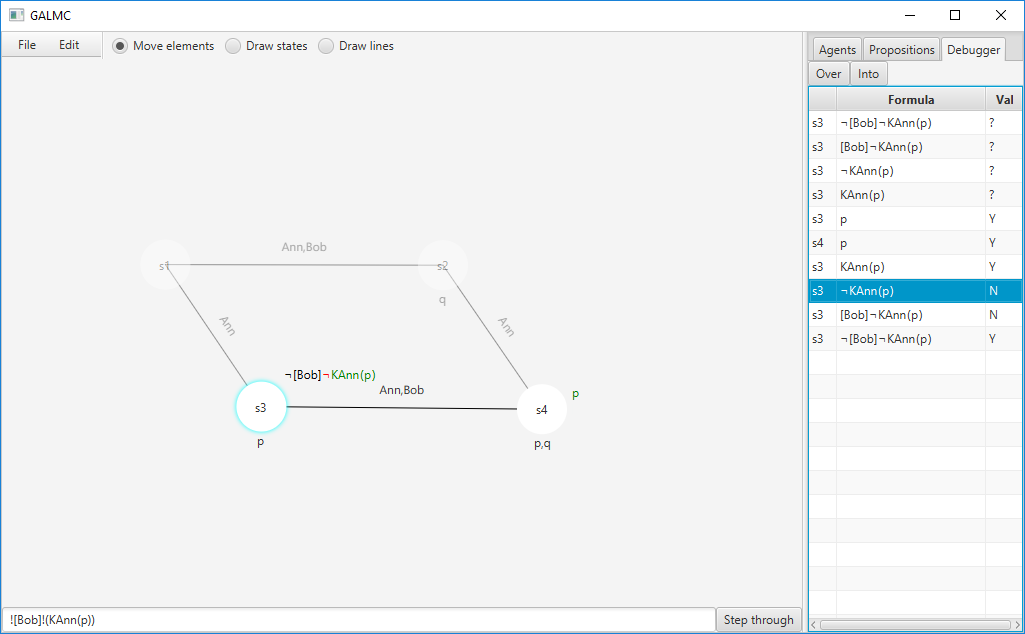
\includegraphics[width= \textwidth]{MCGALBasicChecking.png}
\end{figure}

As the tool provides a view of the model, it also updates this view by highlighting what the model it is currently checking against looks like, by graying out any states that have been filtered out by a model update, such as each formula extension a coalition can announce, which is what is being displayed in Figure \ref{fig:basicGalChecking}. In this example, we are checking state s3 against the formula $\neg [Bob]\neg KAnn[p]$ translating to: 'It is not the case that Bob is unable to make Ann know $p$' or more simply in its dual form: 'Bob is able to make Ann know p'. In the figure we can see that as Bob is able to reduce the model to only states where $p$ holds, Ann also trivially knows $p$ in this updated model, satisfying our original formula. In our somewhat trivial example, the tool ended up only trying a single model as it only had to find a single extension that made the formula true. If we were to check an unnegated group announcement formula, it would have to check every possible formula extension announceable by the given coalition, but it would also visualize all of these updated models until it finds one where the formula does not hold, giving the user insight into the coalitions capabilities. Note that the previous example could also have been made easier by rewriting the formula as $\dia{Bob}KAnn[p]$, but unfortunately the tool does not (yet) support diamond operators. 
